%
% Copyright (c) 2024
% Rémy Hubscher - <hubscher DOT remy AT gmail DOT com>
%
% This file may be distributed and/or modified under the terms of 
% the Apache v2 licence
% 

\documentclass{beamer}

\usetheme[shownavigation={false},  % true | false
          utbmlogo={LogoAAA.png},
          logo={logo.png},
          titlepageimage={titleimage.png},
          header=fullnav,          % fullnav | shortnav | utbm
          suiveur={Franck BERTAGNINI},
          dept={Formation FI (A)}
        ]{UTBM}

\usecolortheme{Terra}

\usepackage[francais]{babel}
\usepackage{datetime}  
\usepackage[T1]{fontenc}
\usepackage{lmodern}

\author{Rémy HUBSCHER} 

\begin{document}
  \title[Briefing Long — Conditions VMC]{Les Conditions du vol à vue en France (VMC)}
  \subtitle{Briefing Long — Conditions VMC}
\date{\today} 

\begin{frame}[plain]
  \titlepage
\end{frame}

\begin{frame}{Objectifs}
  Étudier les conditions VMC minimales réglementaires pour définir la
  météo minimale d'un vol prévu.
\end{frame}

\begin{frame}{Utilité}
  \begin{itemize} 
    \item Savoir dire si le vol prévu est réglementaire ; \pause
    \item Voler en toute sécurité en évitant les traffics, obstacles et les nuages ; \pause
    \item Pouvoir naviguer avec des points de repère au sol (cheminement, points tournant, points d'entrée) ; \pause
    \item Prévenir des situations dangereuses ; \pause
    \item Garantir sa séparation avec les traffics IFR.
  \end{itemize}  
\end{frame}

\begin{frame}{Rapport}
  \textbf{En voiture}
  
  \begin{itemize}
    \item Qu'elle est la limite de vitesse sur l'autoroute ? \pause sous pluie ? \pause
    \item Qu'elle est la limite de vitesse lorsque la visibilité est inférieure à 50 m ? \pause
    \item Qu'impose la loi montagne vis à vis des roues des voitures ? \pause
  \end{itemize}

  \vspace*{1em}
  En voiture on a une réglementation pour garantir la sécurité en fonction des conditions du jour.
  \pause
  
  \vspace*{1em}
  C'est pareil en avion.
\end{frame}

\section{Questions}
\begin{frame}{Les espaces aériens}
  \textbf{Qu'elles sont les classes d'espace aérien ?}

  \pause
  \begin{figure}
    \centering
    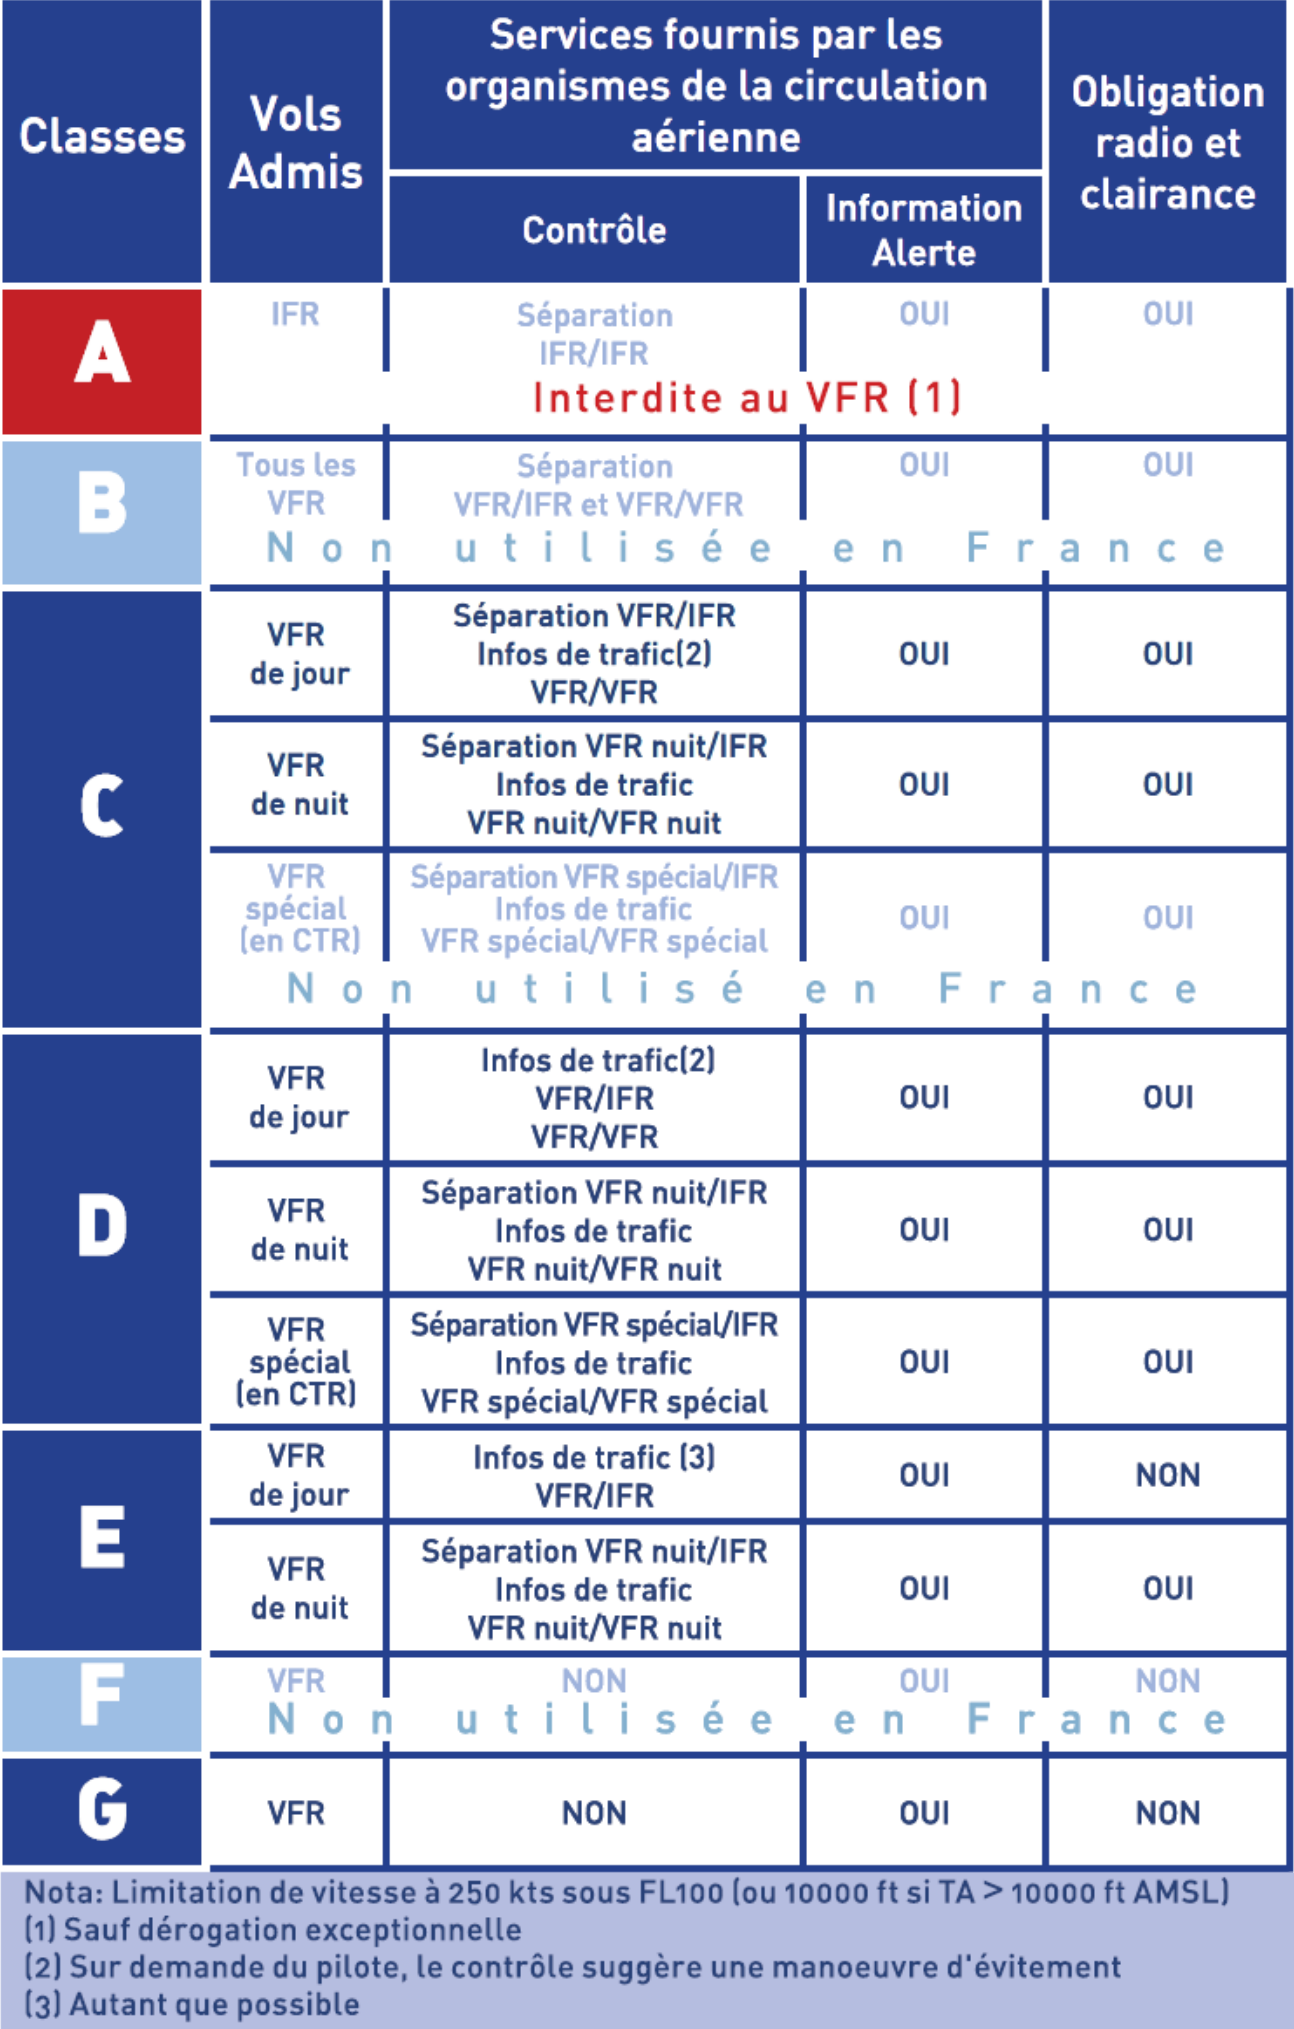
\includegraphics[scale=0.43]{images/espaces-aeriens.png}
  \end{figure}
\end{frame}

\begin{frame}{Le calage altimétrique}
  \textbf{Qu'est-ce que le QNH et le QFE ?}
  
  \begin{itemize}
    \item QNH : Calage altimétrique donnant l'altitude par rapport au niveau moyen de la mer (AMSL) \pause
    \item QFE : Calage altimétrique donnant la hauteur par rapport au sol (AGL)
  \end{itemize}

\end{frame}

\begin{frame}{Thème}
  \tableofcontents
\end{frame}

\section{Définitions}
\begin{frame}{Définitions}
  \LARGE{Définitions}
\end{frame}

\begin{frame}{VMC — Visual Meteorological Conditions}
  Le terme VMC est définie dans l'Annexe 2 des règles de l'air de l'OACI :

  Il y est dit que tous les vols VFR doivent respecter les minimas du tableau ci-dessous :

  \pause
  \begin{figure}
    \centering
    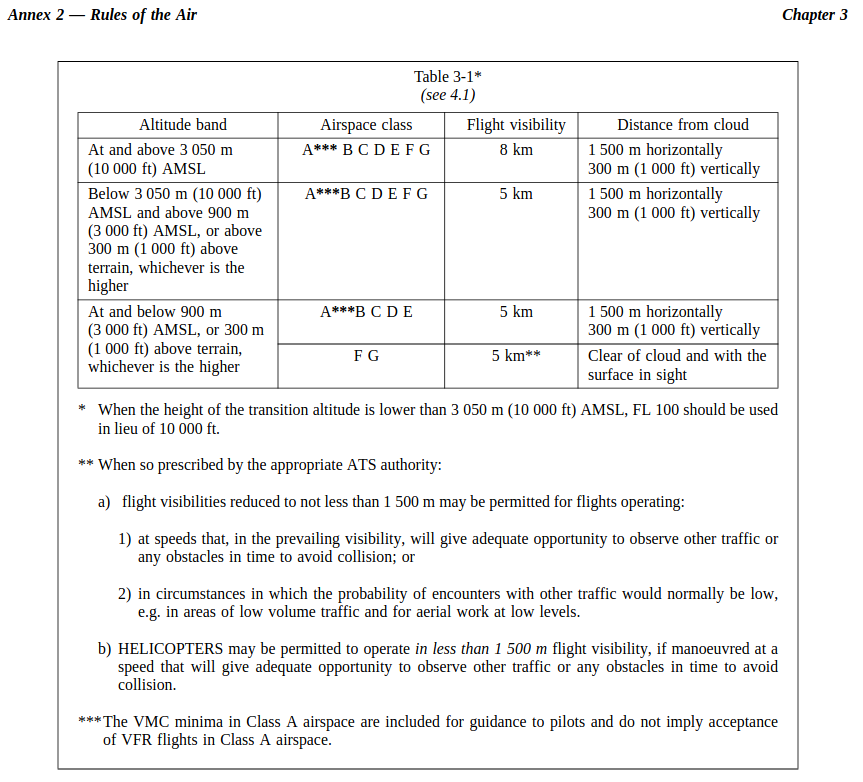
\includegraphics[scale=1]{images/rule-of-air.png}
  \end{figure}
\end{frame}

\begin{frame}{VMC — Visual Meteorological Conditions}
  Cette définition est reprise pour la définition européenne SERA.5001 et Française SERA.FRA.5001 :

  \pause
  \begin{figure}
    \centering
    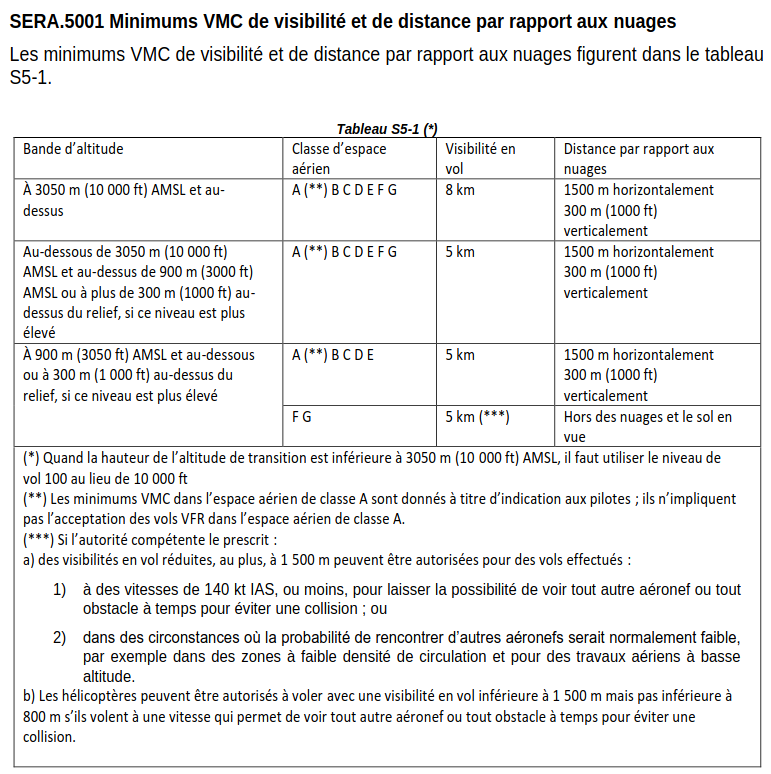
\includegraphics[scale=1]{images/sera.5001.png}
  \end{figure}
\end{frame}

\begin{frame}{IMC — Instrument Meteorological Conditions}
  Le terme IMC quant à lui signifie, les conditions météorologiques qui sont inférieures aux conditions VMC.

  \pause
  \begin{figure}
    \centering
    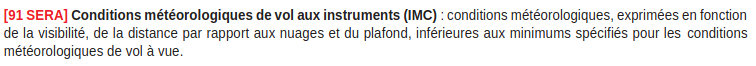
\includegraphics[scale=1.8]{images/sera.imc.png}
  \end{figure}

  \pause

  On constate que contrairement à la croyance, IMC ne veut pas dire
  qu'on est entré dans un nuage, mais que les conditions VMC ne sont
  pas réunies.
\end{frame}


\begin{frame}{La surface S}
  Les conditions VFR se décompose en 3 grandes règles :

  \begin{itemize}
    \item Les règles en classe Golf, sous la surface S, \pause
    \item Les règles en classe Golf, sur la surface S, \pause
    \item Les règles en espace aérien contrôlé.
  \end{itemize}

\end{frame}


\begin{frame}{La surface S}
  La surface S correspond à l'espace entre :

  \begin{itemize}
    \item Le sol et la plus haute valeur entre : \pause
    \item 1000 ft AGL (QFE), et 3000 ft AMSL (QNH). \pause
  \end{itemize}

  \pause
  \begin{figure}
    \centering
    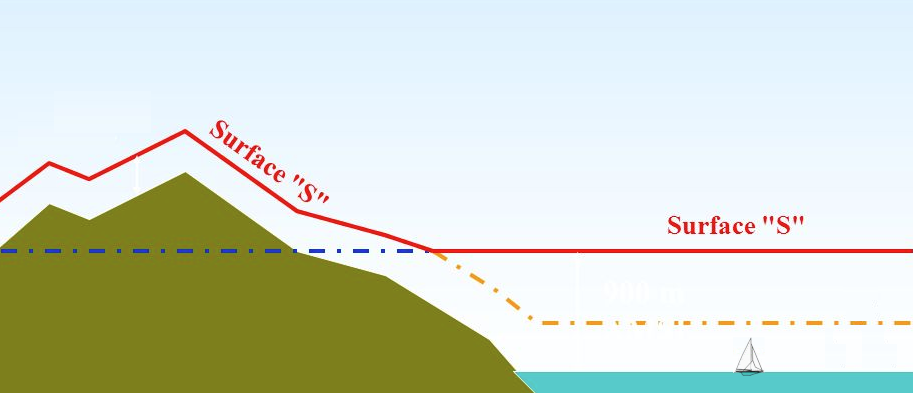
\includegraphics[scale=1.2]{images/surface-s.png}
  \end{figure}
  
\end{frame}

\end{document}
